\title{\textbf{Text Analytics} \\ 3\textsuperscript{rd} Assignment}
\author{
        Kyrkos Konstantinos - p3351907\\

        
}
\date{\today}


\documentclass[10pt]{article}

\usepackage{tikz}
\usetikzlibrary{shapes,backgrounds}
\usepackage{fancyhdr}
\usepackage{amsmath}
\usepackage{amssymb}
\usepackage{listings}
\usepackage{float}
%\usepackage{hyperref}
%\usepackage{graphicx}
\usepackage{enumitem}
\graphicspath{ {./images/} } 
%\usepackage[showframe]{geometry}
\usepackage[hyperfootnotes=false]{hyperref}
\fancypagestyle{headings}{
\cfoot{\thepage}
}
\usepackage{multirow}
\usepackage{verbatimbox}
\begin{document}
\maketitle

This report is one of the two deliverables which we provide as a solution to the 3rd Assignment for the course of Text Analytics of the MSc in Data Science at Athens University of Economics and Business. 

Below we provide an overview of what we have created, explanations for methods and patterns used, descriptions and opinions on tools, algorithms and practices.

\section*{Exercise 9 - Sentiment classifier using MLP}

For the purpose of this excercise we have implemented a sentiment classifier for the tweet texts extracted from the Twitter social network using Multi-Layer Perceptrons. We decided to occupy ourselves with Exercise 9 instead of Exercise 10, as this third assignment was the natural development of the second assignment, only this time with MLPs and thus we could examine, how better our sentiment classifier could become using MLPs. The dataset we used again is named "Sentiment140" and contains 1.6 million tweets.

\subsection*{Packages and Datasets}
We start this assignment by installing all missing packages and then we mount our Google Drive in order to load and save data without losing them between runtime sessions. We then, import all the libraries we will later use in our code and download, unzip and load our \href{https://fasttext.cc/docs/en/crawl-vectors.html}{fastext word embeddings}. These embeddings are pre-trained word vectors for 157 languages, trained on Common Crawl and Wikipedia using fastText. These models were trained using CBOW with position-weights, in 300 dimensions , with character n-grams of length 5, a window of size 5 and 10 negatives. Next we download and unzip our dataset from the following link provided by the Stanford University.

\begin{itemize}
\item
\href{http://cs.stanford.edu/people/alecmgo/trainingandtestdata.zip}{Sentiment140 Link}.
\end{itemize}

Moving on, we load the data to a dataframe choosing "ISO-8859-1" for decoding as there were major failures when using Unicode, or "UTF-8" . After having a closer look at our data, we drop the extra columns, that are not usefull for our assignment, as "text" and "sentiment" are the only columns needed in our case. Our dataset uses the "sentiment" column to denote the sentiment of the tweet, using "0" for negative, "2" for neutral and "4" for positive sentiment. As we discovered that our dataset although it supports three labels, contains only two of them (positive/negative), we change the value of sentiment "4" to "1" in order to give our results a binary look. We then, add a block of code, where we can lighten our colab storage and remove files we won't be needing in the following sections. In the following code block, we print the count of the column "sentiment" and check how many values are there from each category. As we can see, in our case we only have negative and positive values equally divided, thus a balanced dataset. 

\subsection*{Data Preparation}

Next, we create two dictionaries which will later help us clean and manipulate our dataset better. The (\textcolor{red}{\textit{load\_dict\_smileys}}) maps most commonly used smiley faces with a description and (\textcolor{red}{\textit{load\_dict\_contractions}}) maps most commonly used contraction of words to the corresponding non-shortened phrases.

Next, we create a function (\textcolor{red}{\textit{tweet\_cleaner}}) cleaning our text from characters that are not usefull for the purposes of our assignment. The method is mainly based on regular expressions which help us achieve our goal. Some examples of cases and characters we want to remove are: references to other users via @ character, links to websites, single character words, hashtags, number and finally multiple spaces. We also occupy ourselfs with cases of html tags left in our texts and we care about removing faulty characters which might have been the outcome of the decoding process of the text. Next, we utilize the two dictionaries we created to map contractions/slang and smiley faces in actual words with the same meaning. 
Furthermore, we replace three or more repetitions of letters with only two in order for multiple misspelled words to map in a unique one. 
Finally, we replace emojis with their corresponding word meaning and lematize each word to merge multiple versions of the same words into one. 
\footnote{https://towardsdatascience.com/fasttext-sentiment-analysis-for-tweets-a-straightforward-guide-9a8c070449a2}.
For example the tweet:
\begin{figure}[H]
\centering
\caption{Raw tweet}

\includegraphics[width=0.7\textwidth]{tweet_raw.png}
\end{figure}
will be mapped to the following word sequence:
\begin{verbatim}
lot of rock thumb up fell fromm the sky smiley 
he will consider taken an umbrella love
\end{verbatim}

Moreover, after taken a subset of our data we shuffle it, because we have noticed that the positive sentiment tweets are placed lower on the dataset and we don't want that messing with our outcome \footnote{shuffling the sentences makes the training more unbiased}. For each of the tweets in our sample, we apply our cleaning function and then we keep only the rows which containt text after the process described (empty tweets will be dropped). 

Next, we create a new function named  (\textcolor{red}{\textit{text\_centroid}}) that transforms the tokenized words into word embeddings and then create a centroid as the average of the word embeddings in each tweet. After the process is finished, some centroids end up without values and we drop them as well. 

\[
T = \frac{1}{d}\sum_{i=1}^{d}w_i
\]

\subsection*{Dataset Splitting}

In the following code block, using the dataset we have manipulated until this point, we split it into three different sets:
\begin{itemize}
\item
The largest set, will be our training set, consisting of the \textbf{80\%} of the dataset. 
\item The next part, will be the development set, which will be used for hyperparameter tuning and consists of the \textbf{10\%} of the dataset. 
\item The final part, will be our test set consisting of the remaining \textbf{10\%} of our dataset.
\end{itemize}

Next, we finalize our training set, creating a numpy array by stacking all our centroids together and by keeping only the sentiment column from our dataframe turned into a list.
We repeat the same process for all of our datasets.

\subsection*{Some statistics on the dataset}

In order to understand our dataset better, we continue with extracting some statistics from our dataset. First, we get the document length per sentiment and as we can see the negative sentiment category has 1 more word on avergage, compared to the positive category. That may, or may not play a significant role in identifying the sentiment of the text. 

\subsection*{Average word count per class }
\begin{tabular}{ |p{3cm}|p{3cm}|  }
\hline
 Class 0 & $13.5$\\\hline
 Class 1 & $12.38$\\  
\hline
\end{tabular}
\bigskip  

Next, we print the total number of documents in our subset of the initial dataset. Interesting enough here, we started with 100.000 rows but we ended up with 99.765 due to data cleaning. \footnote{For the purpose of this exercise we did not use the whole dataset, consistinf of 1.6 million tweets. Instead, we used a subset of 100000 tweets, which we believe is sufficient enough for the purpose of this exercise, without consuming an enormous amount of resources}

Having seen the number of total documents interesting would be to see the size of each dataset. We can see the corresponding sizes below. Of course that process is only made, to verify our calculations when splitting our dataset.

\subsection*{ Sizes for each set }
\begin{tabular}{ |p{5cm}|p{3cm}|p{3cm}|  }
\hline
 Training set & $79812$\\ \hline
 Development set &   $9975$\\ \hline
 Test set &   $9976$\\  
\hline
\end{tabular}
\bigskip 

\newpage
\subsection*{Classification metrics}

We created our own function (\textcolor{red}{\textit{get\_scores}}) that calculates the following metrics, for user-defined classification thresholds as well as for all the classes:

\[
\text{Precision} = \frac{\text{TP} }{\text{TP} + \text{FP} }
,\quad  \text{Recall} = \frac{\text{TP} }{\text{TP} + \text{FN} }
,\quad  \text{F}_1 = \frac{2\times \text{Precision}\times \text{Recall}}{ \text{Precision} + \text{Recall}}\quad \footnote{We checked whenever the denominator was zero, and set the entire score to zero, in order to avoid arithmetic errors}
\]

Similarly we use macro-averaging to get a more robust estimate for all the classes
\begin{align*}
\text{Macro - Precision} &= \frac{1}{n}\sum_{i=1}^n{\text{Precision}_i } \\
 \text{Macro - Recall} &= \frac{1}{n}\sum_{i=1}^n{\text{Recall}_i } \\
 \text{Macro - F}_1 &= \frac{1}{n}\sum_{i=1}^n{\text{F1}_i }
\end{align*}

\bigskip
\subsection*{Classifiers}

Moving on to the main part of the assignment, we now provide a MLP we found through experimentation, but before developing the MLP classifier we present two linear classifies used in the previous assignement. The first is a baseline majority classifier and the second is our best probabilistic classifier from the second assignment. The purpose of presenting these classifiers is to see how well, we can classify our tweets to the correct sentiment and how can our MLP increase our scores when classifying.

Our baseline classifier like the last time is, the \href{https://scikit-learn.org/stable/modules/generated/sklearn.dummy.DummyClassifier.html}{DummyClassifier} from sklearn, which we parameterize to always return the most frequent result. We fit our training data on the classifier and then utilizing the methods we have previously created, we get our results. We present our results below: 

\bigskip
All the scores presented bellow are measured for a classificiton threshold $t = 0.5$:

\subsubsection*{Baseline classifier}
\begin{tabular}{ |p{2cm}||p{3cm}|p{3cm}|p{3cm}|  }
 \hline
 \multicolumn{4}{|c|}{\textcolor{teal}{Training set}} \\
 \hline
  & \textbf{Precision} &  \textbf{Recall} & $\textbf{F}_1$\\
 \hline
 Class 0 & 0    &  0 &   0 \\
 Class 1 & 0.501 & 1 & 0.668\\  \hline
 Macro & 0.251 &  0.5 &  0.334\\
 \hline
  \hline
  
   \multicolumn{4}{|c|}{\textcolor{teal}{Development set}} \\
 \hline
  & \textbf{Precision} &  \textbf{Recall} & $\textbf{F}_1$\\
 \hline
 Class 0 & 0 & 0 &  0 \\
 Class 1 & 0.502 & 1  & 0.669\\  \hline
 Macro & 0.251 &  0.5 &  0.334\\
 \hline
  \hline
  
  \multicolumn{4}{|c|}{\textcolor{teal}{Test set}} \\
 \hline
  & \textbf{Precision} &  \textbf{Recall} & $\textbf{F}_1$\\
 \hline
 Class 0 & 0   & 0 &  0\\
 Class 1 & 0.501  & 1  & 0.668\\  \hline
 Macro & 0.251 &  0.5 & 0.334\\
 \hline
 \hline
\end{tabular}


For our next classifier we chose the \href{https://scikit-learn.org/stable/modules/generated/sklearn.linear_model.SGDClassifier.html}{SGDClassifier} from sklearn. This is a set of linear classifiers with SGD training. For the loss parameter of the classifier we choose "log" which gives us logistic regression and so in total we have basically Logistic regression as the classifier, but using SGD ( Stohastic Gradient Descent) training. This classifier as it was also mentioned above was the one to give the best classification results in the last assignment. Then, we train our model and again utilizing our method, we get the scores of the model on all three of our sets. We present our results below:

\subsubsection*{Logistic Regression classifier}
\begin{tabular}{ |p{2cm}||p{3cm}|p{3cm}|p{3cm}|  }
 \hline
 \multicolumn{4}{|c|}{\textcolor{teal}{Training set}} \\
 \hline
  & \textbf{Precision} &  \textbf{Recall} & $\textbf{F}_1$\\
 \hline
 Class 0 & 0.744 & 0.738 & 0.741 \\
 Class 1 & 0.742 &  0.747 & 0.744 \\  \hline
 Macro & 0.743 & 0.743 & 0.743 \\
 \hline
  \hline
  
   \multicolumn{4}{|c|}{\textcolor{teal}{Development set}} \\
 \hline
  & \textbf{Precision} &  \textbf{Recall} & $\textbf{F}_1$\\
 \hline
 Class 0 & 0.741 & 0.737 & 0.739 \\
 Class 1 & 0.74 & 0.744 & 0.742 \\  \hline
 Macro & 0.741 & 0.741 & 0.741\\
 \hline
  \hline

  \multicolumn{4}{|c|}{\textcolor{teal}{Test set}} \\
 \hline
  & \textbf{Precision} &  \textbf{Recall} & $\textbf{F}_1$\\
 \hline
 Class 0 & 0.74 & 0.739 & 0.74 \\
 Class 1 & 0.741 & 0.742 & 0.741\\  \hline
 Macro & 0.74&  0.74 & 0.74\\
 \hline
 \hline
\end{tabular}
\bigskip

\newpage
\subsubsection*{MLP classifier}

Next, we create four new methods which will helps us retrieve results from the Keras model we will create in the following code blocks. These methods will give us batch-wise average for recall, precision, f1 and accuracy. 

In the following code block, we turn our sentiment columns from lists to numpy arrays and then stack them with another column. This column contains the opposite result of the true (if the right one is "0", the new column will contain "1"). We perform this transformation in order for the \textbf{predict()} method of our two-output keras classifier to give us two results, the probability that the data row belongs to label ''0'' and the probability that belongs to label ''1''. We make sure that these probabilities sum to one.

\[
y_{new} = \begin{bmatrix} 1-y & y  \end{bmatrix}^T =  \begin{bmatrix} 1 & 0\\ 0 & 1\\ 0  & 1\\ \vdots \\ 1 & 0 \end{bmatrix}
\]

Now it is time to create a new Sequential model using Keras. We initially add a Dense layer with 256 units and activation function relu, followed by a Dropout layer with 0.5 rate.\footnote{The dropout layers help our classifier from overfitting}. Following, we added the same two layers for a second time only this time the Dropout Layer has a rate of 0.3 . Then add a Dense layer with reduced units (128) using activation function relu, followed by a another Dense layer resulting in 2 units with activation function softmax. This model came after a lot of experimenting with models with more or less layers and also models with larger and smaller dimensions (see \textbf{Appendix A}). We then, compile our model using categorical crossentropy as loss function and the Adam optimizer. Then, we create a set of callbacks which will help us make the model stop if there is no significant improvement in the scores of validation f1 after 5 epochs. 

Finally, we fit our model with our training data using the callbacks we have previously created and set it to run for 30 epochs, evaluating on the development set. 
After training, we get our model evalution scores which we present below, we also utilize our own methods to get scores for all our sets. Below we present our model history graph and also our results below:

\begin{figure}[H]
\caption{Keras model evaluation curves}
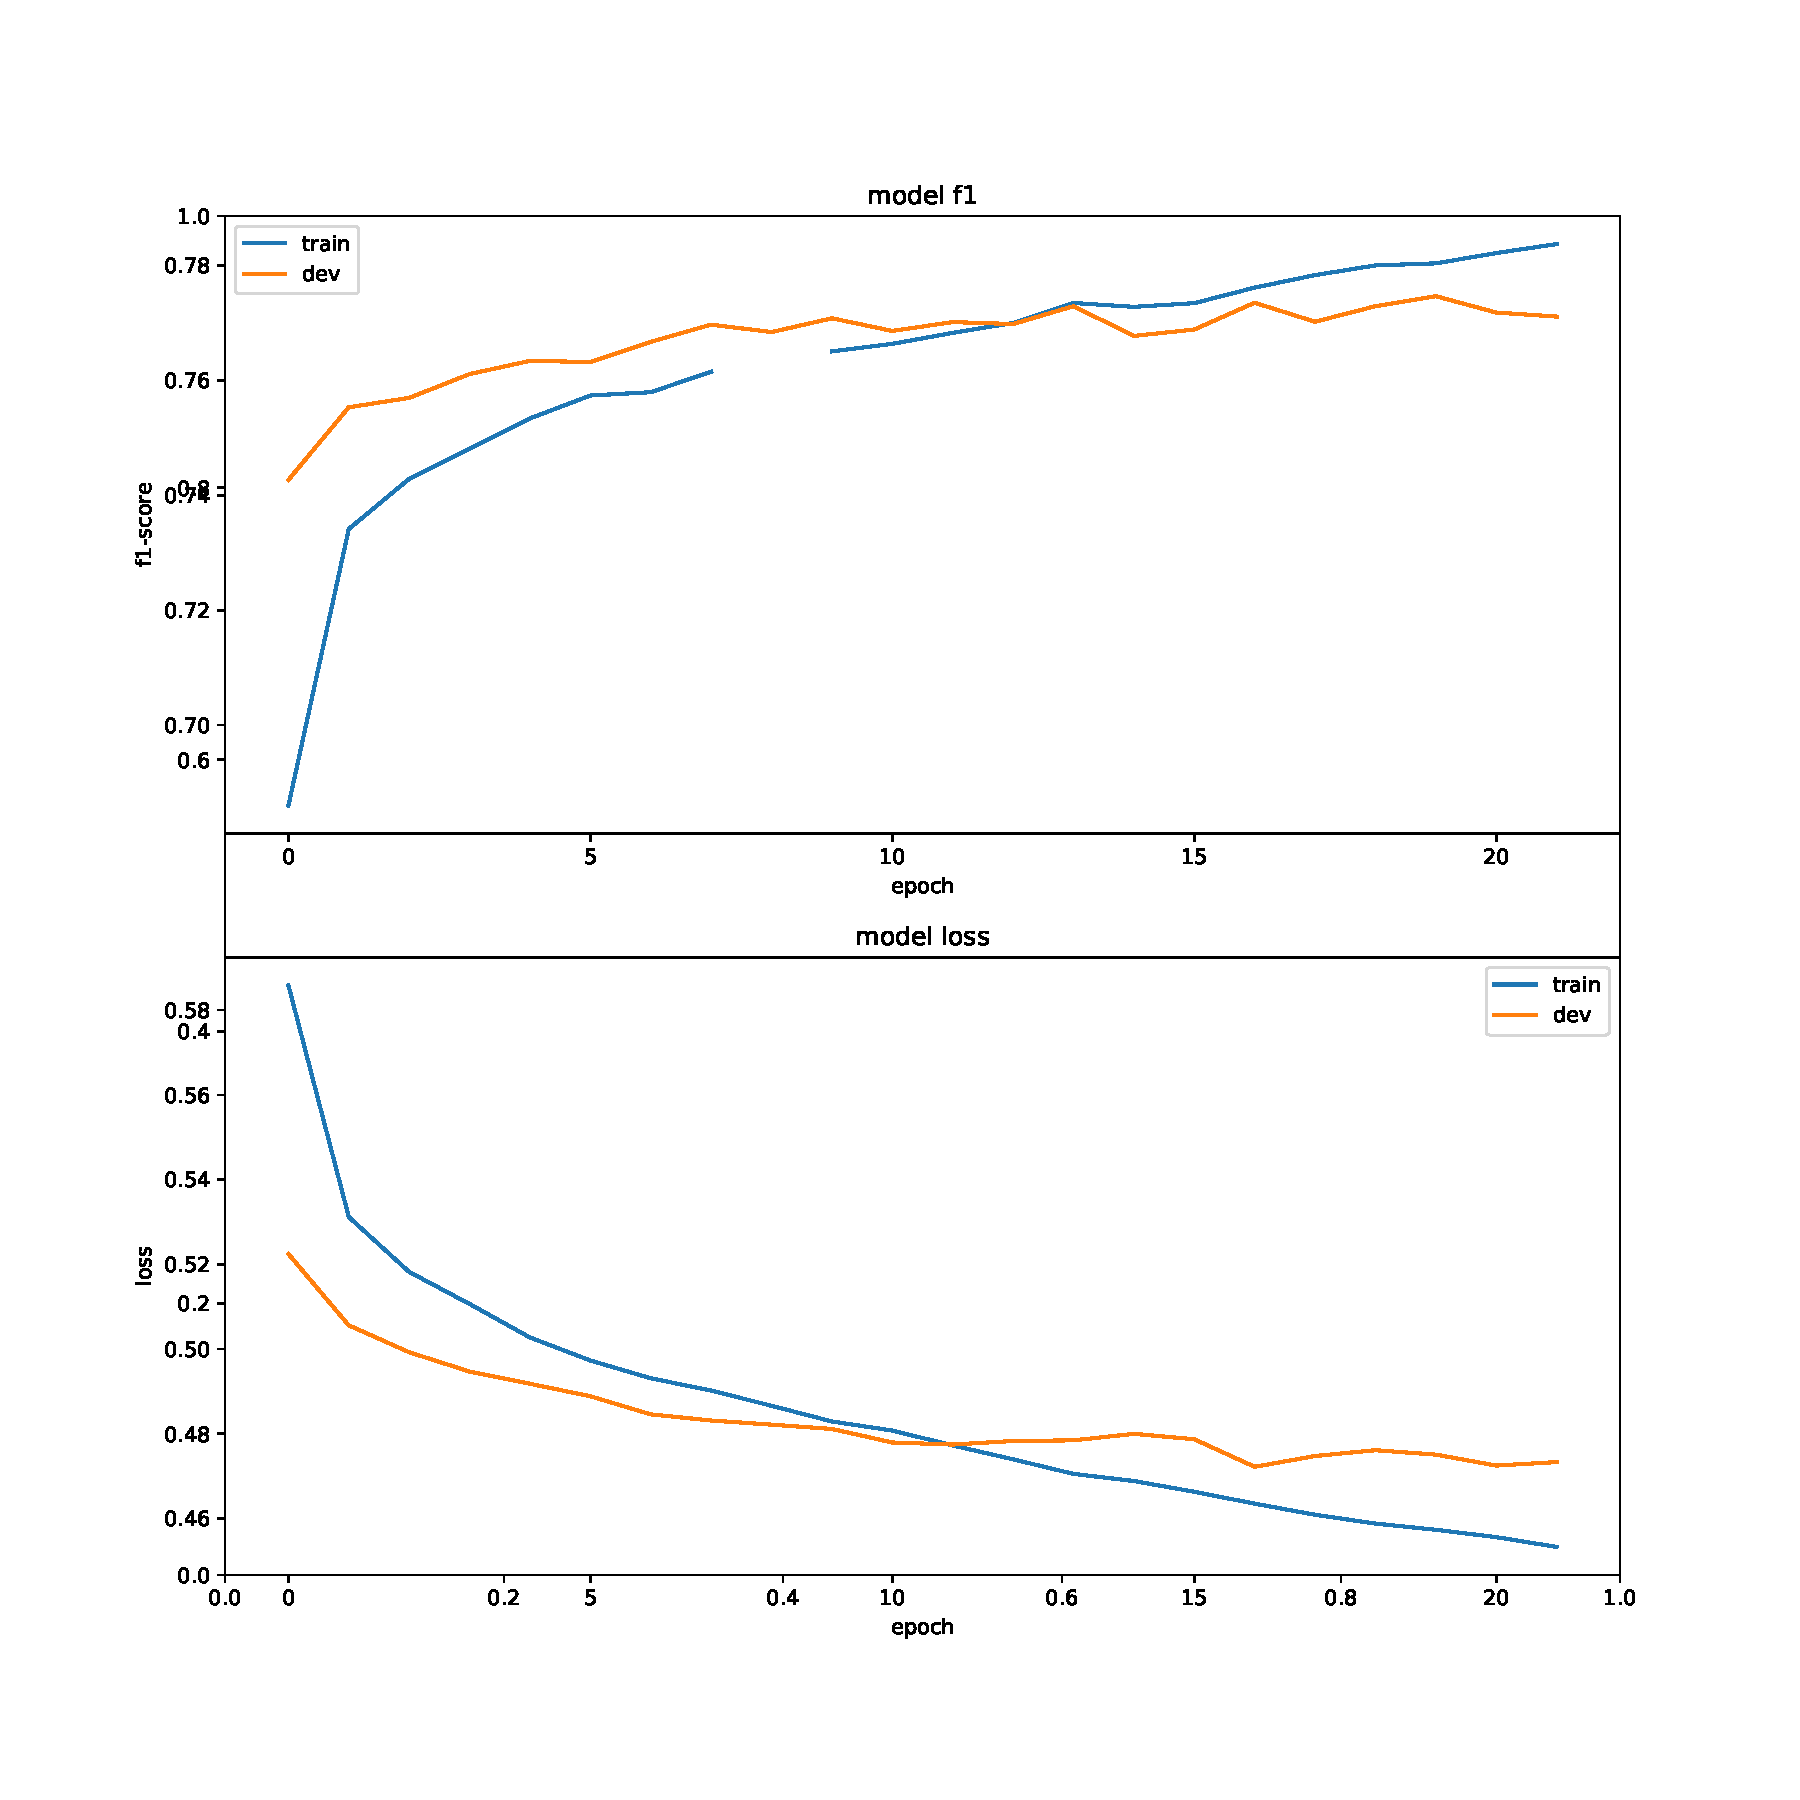
\includegraphics[width=\textwidth]{History_keras.pdf}
\end{figure}

%add final results here
 \subsubsection*{Model Evaluation scores}

\begin{tabular}{ |p{5cm}||p{2cm}|  }
  \hline
 \textbf{Metrics} &  \textbf{Value}\\
 \hline
 Test Binary cross entropy & 0.7815 \\ \hline
 Test precision &0.7815 \\  \hline
 Test f1 & 0.7815 \\ \hline
 Test accuracy & 0.7815 \\
 \hline
 \hline
\end{tabular}

\bigskip
\subsubsection*{MLP scores using our custom metrics}
\begin{tabular}{ |p{2cm}||p{3cm}|p{3cm}|p{3cm}|  }
 \hline
 \multicolumn{4}{|c|}{\textcolor{teal}{Training set}} \\
 \hline
  & \textbf{Precision} &  \textbf{Recall} & $\textbf{F}_1$\\
 \hline
 Class 0 & 0.787 & 0.818 & 0.803 \\
 Class 1 & 0.814 & 0.782 & 0.797 \\  \hline
 Macro & 0.8 & 0.8 & 0.8 \\
 \hline
  \hline
  
   \multicolumn{4}{|c|}{\textcolor{teal}{Development set}} \\
 \hline
  & \textbf{Precision} &  \textbf{Recall} & $\textbf{F}_1$\\
 \hline
 Class 0 & 0.766 & 0.783 & 0.774 \\
 Class 1 & 0.776 & 0.759 & 0.768 \\  \hline
 Macro & 0.771 & 0.771 & 0.771 \\
 \hline
  \hline
  
  \multicolumn{4}{|c|}{\textcolor{teal}{Test set}} \\
 \hline
  & \textbf{Precision} &  \textbf{Recall} & $\textbf{F}_1$\\
 \hline
 Class 0 & 0.78 & 0.792 & 0.786 \\
 Class 1 & 0.783  & 0.77 & 0.777 \\  \hline
 Macro & 0.782 & 0.781 & 0.781 \\
 \hline
 \hline
\end{tabular}
\bigskip

\subsection*{Precision-recall curves}
Using our own function \textcolor{red}{\textit{get\_scores}}, we implemented \textcolor{red}{plot\_precision\_recall\_curve} that, given a list of thresholds, calculates \textbf{precision} and \textbf{scores} and stores them to lists. Then we calculate the area under curve and plot a figure with those metrics for each threshold value.

\begin{figure}[H]
\caption{Precision Recall Curves: MLP }
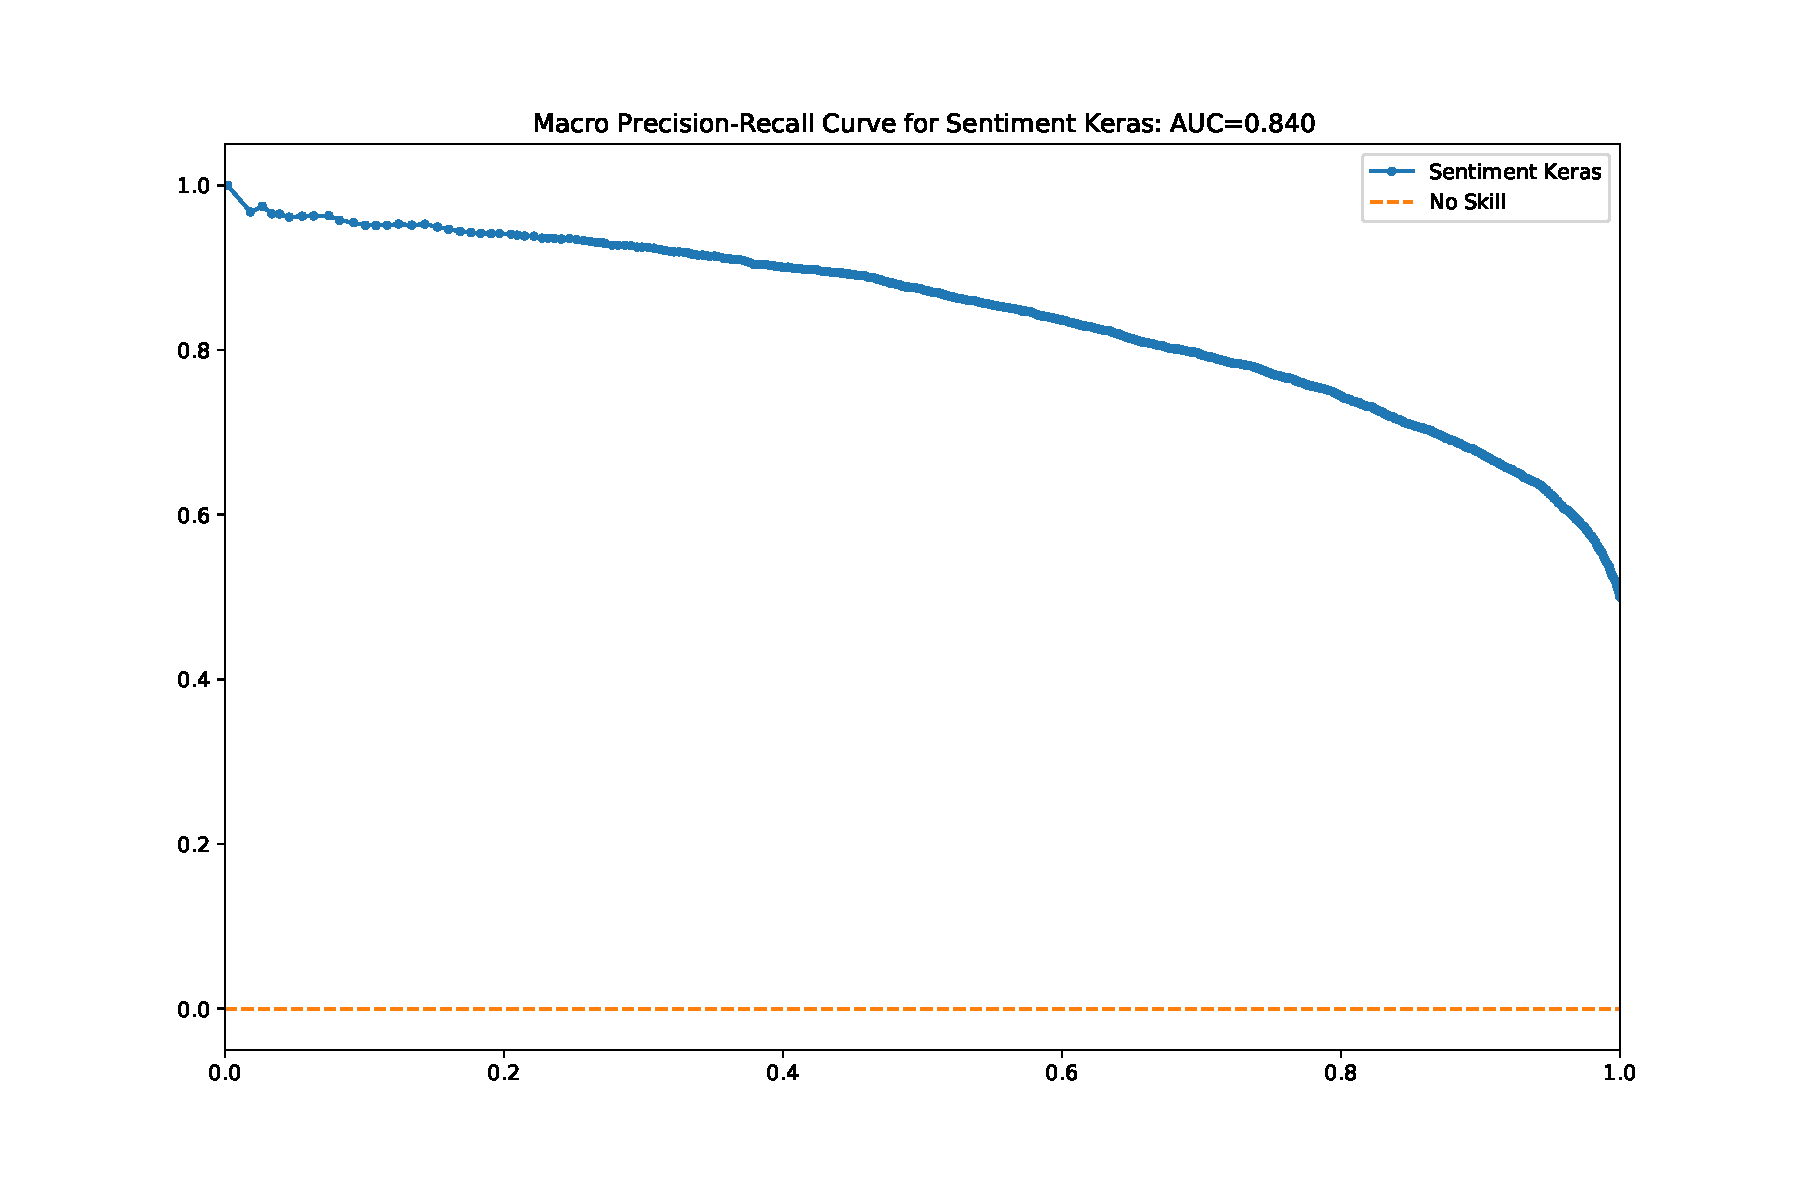
\includegraphics[width=\textwidth]{Sentiment Keras_PR_CURVE.pdf}
\end{figure}

\begin{figure}[H]
\caption{Precision Recall Curves: Logistic Regression}
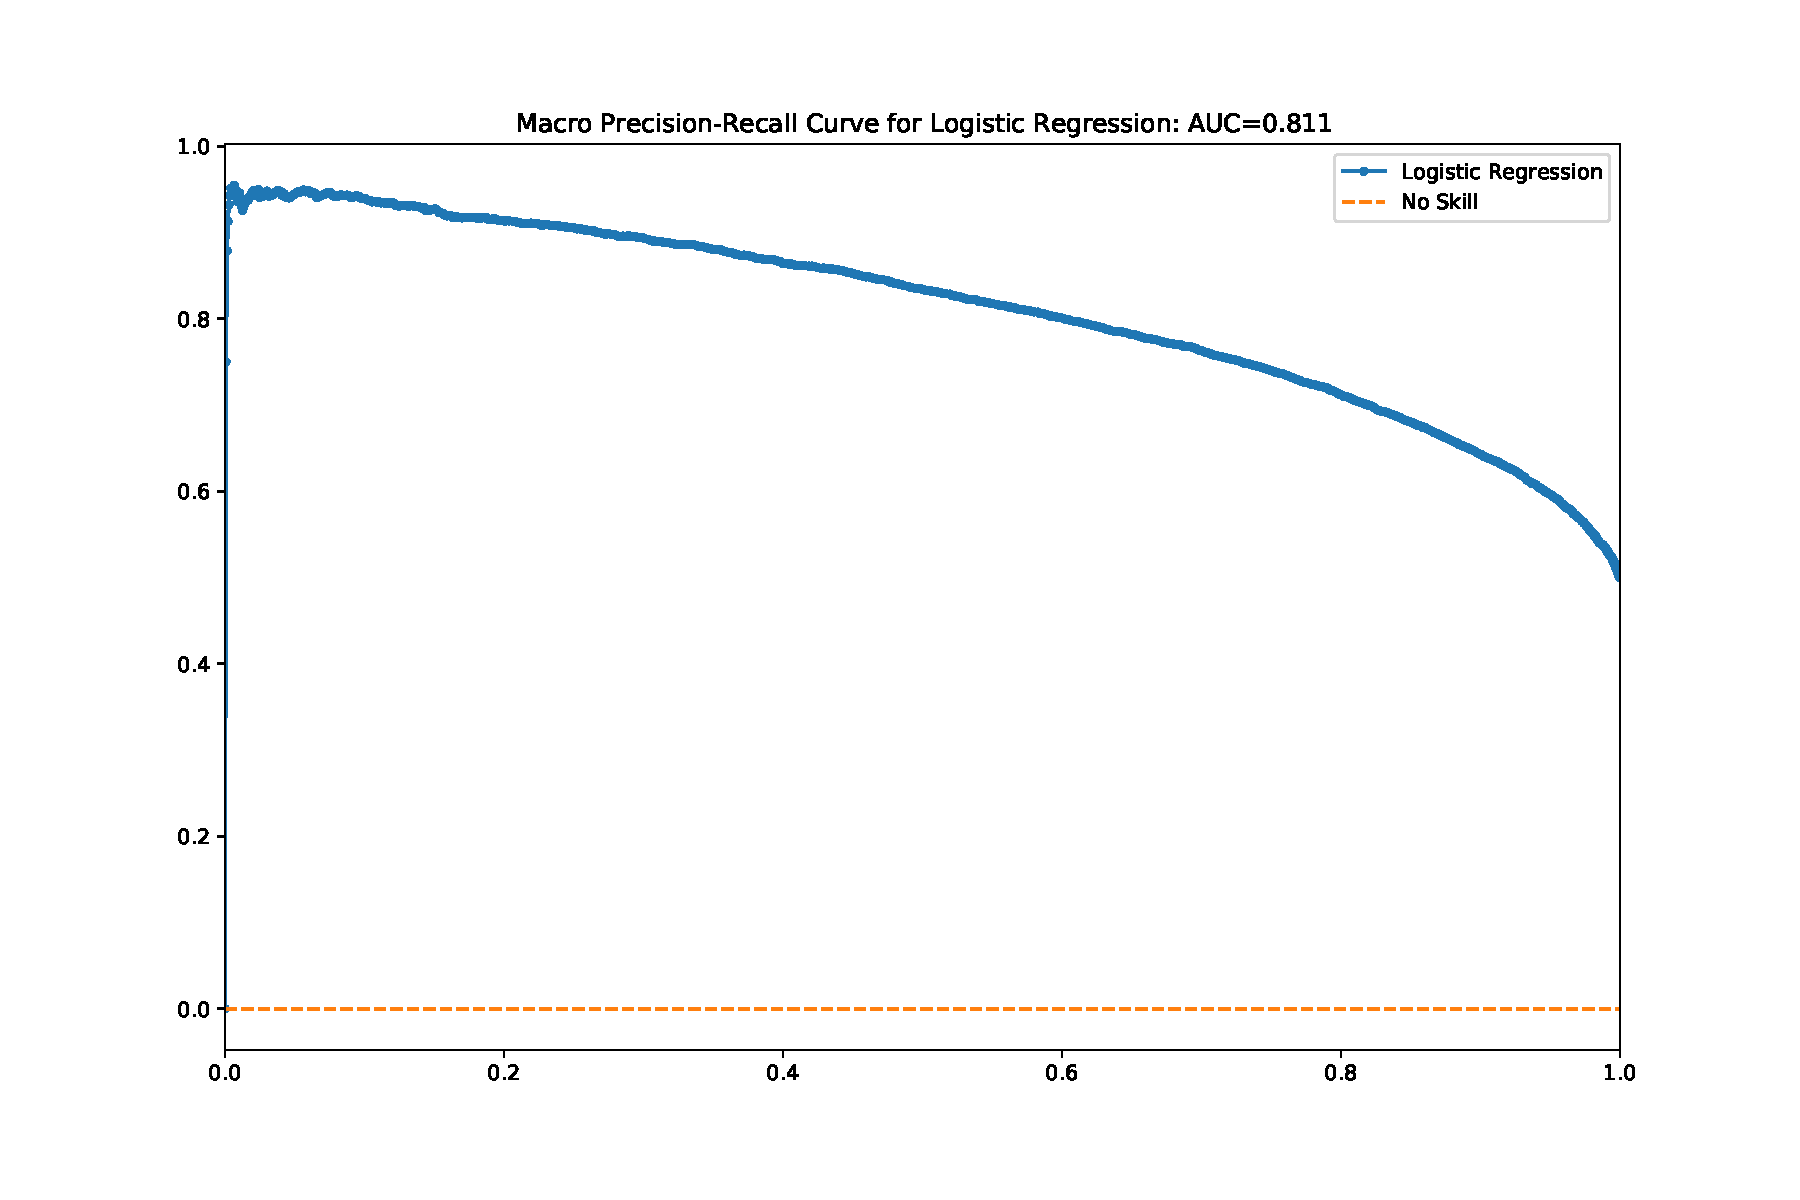
\includegraphics[width=\textwidth]{Logistic Regression_PR_CURVE.pdf}
\end{figure}

\newpage
As we can see, in terms of \textbf{AUC} (area under curve), the \textbf{MLP classifier} is the best among the others and also as we saw above, it scored better than all other classifiers in all previous sections metrics. This proves that these kind of figures have great value when one evaluates different classifiers and also, combined with other metrics, can provide userfull information for safe conclusions. As we know, just because one classifier outscored the other on a certain threshold, that doesn't mean that it is the overall best classifier, but in our case all data point to that direction.

\subsection*{Learning curves }
Moving on, although it was not a deliverable for the exercise, we thought it was interesting to examine the learning curves from the MLP. Utilizing the graph below, we can comment on the following. The model we have created seems to have great capacity and initially seems to overfit as we have provided only a fraction of our original data. But we can see that as we increase the volume of our data, our model metric seems to drop, thus reduces it's overfit to the data. Finally we seem to have almost the same validation F1 score for all our data and we can also see that maybe our model could have the same result with less data. All in all, we have overfitted our data, but we also delivered the best macro f1 score from all the other classifiers as well.

\begin{figure}[H]
\caption{Learning Curves: MLP }
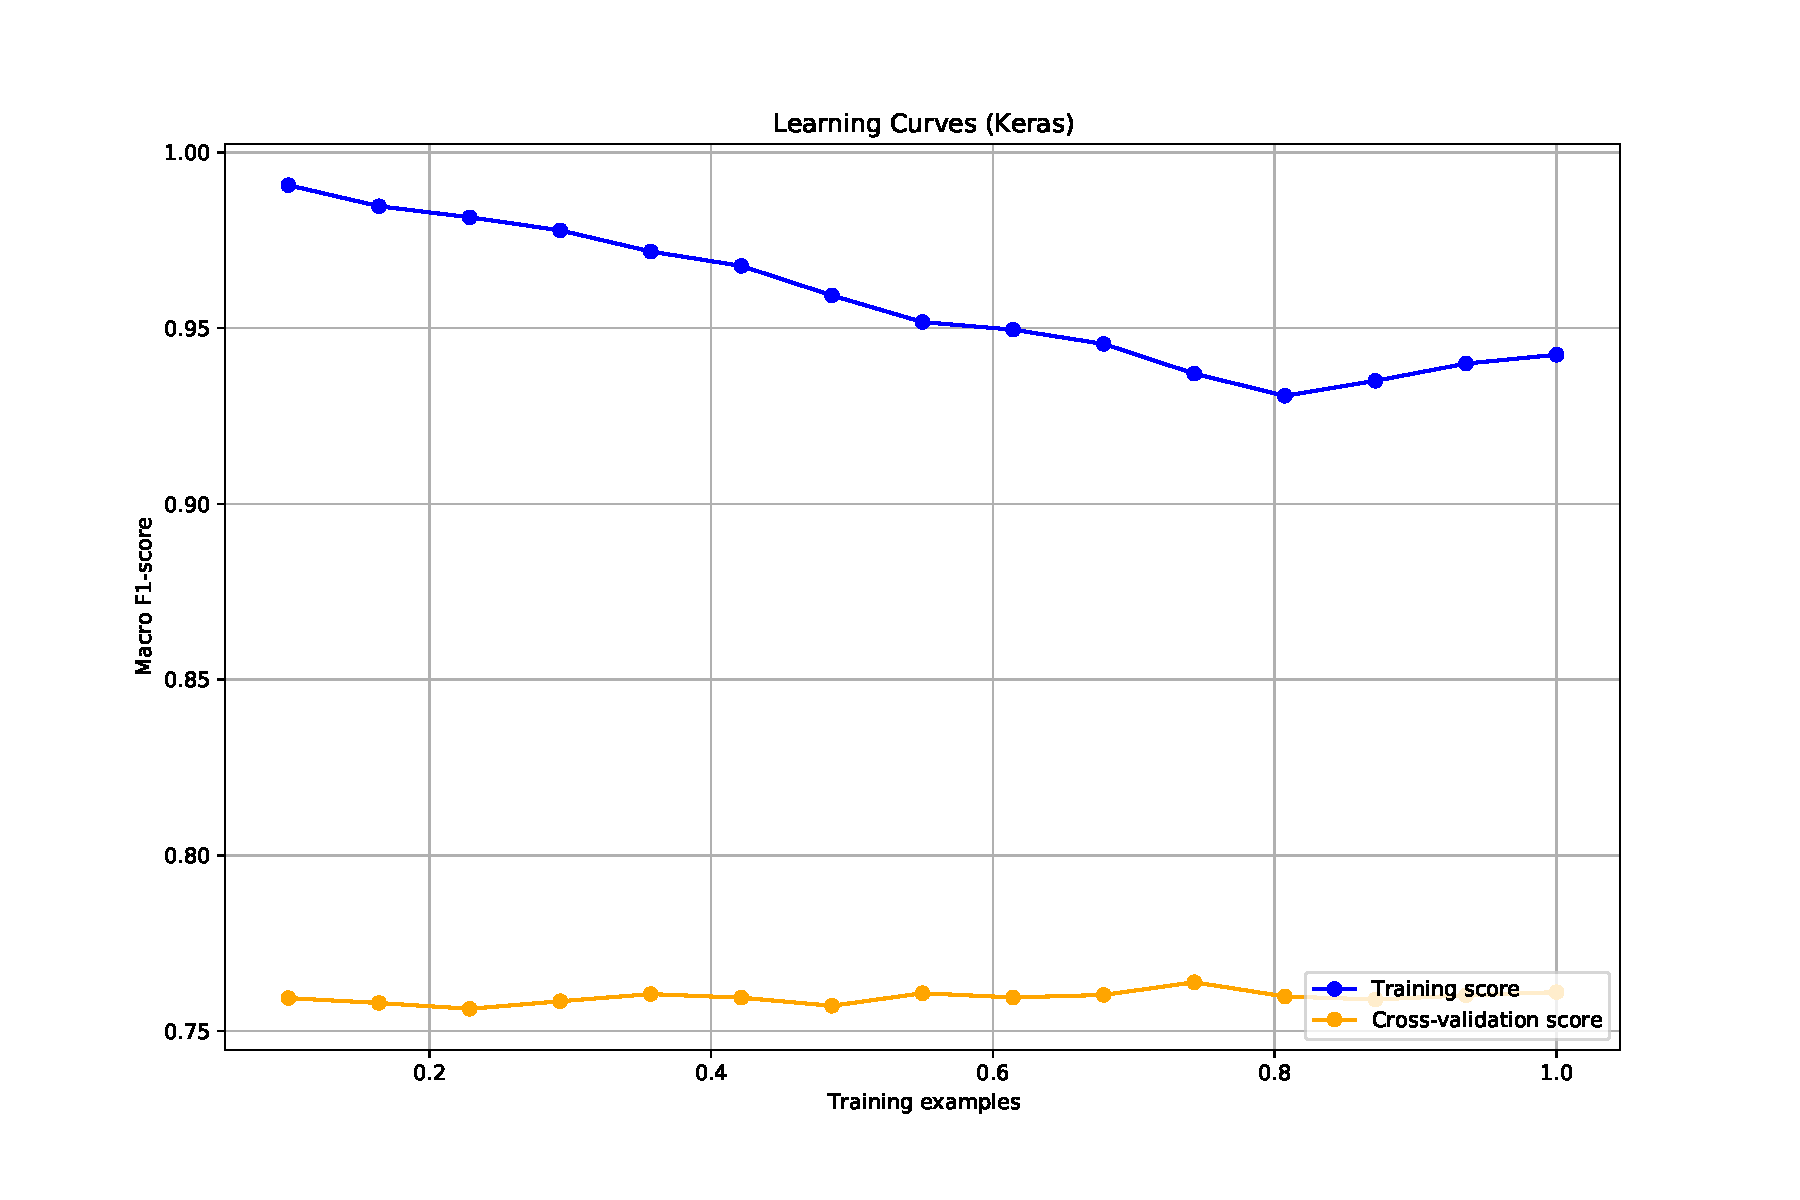
\includegraphics[width=\textwidth]{Learning Curves (Keras).pdf}
\end{figure}

%fix bootstrap
\newpage
\subsection*{Bootstrap statistical significance tests }

In order to derive a safe conclusion on which classifier outperforms the others, we use \textbf{Bootstrap Hypothesis Tests}.
Let A the best classifier in terms of some metric on a test set and B another classifier that we want to compare it with. 
The main idea here is that we assume the null hypothesis ($H_0$) is that the difference between the two classifiers, in the chosen metric, would be zero. 
The alternative hypothesis ($H_1$), is that indeed, there is a significant difference between the evaluation scores not a random fluke. \\
Let $\delta(x) = \text{Macro-F1}_\text{A} - \text{Macro-F1}_\text{B}$, be the difference calculated on all the test set.\\

We state the following hypotheses as the null and alternative one:
\[ 
H_0: \quad \delta(x) = 0 \quad VS \quad H_1: \quad \delta(x) >0
\]
Here, we define $\delta(x^*_i)$ as the differrence between the classifiers on a simulated dataset, sampled from the test set with replacement. 
We calculate the p-value as $p-value \approx\ \frac{s}{b}$ where $s$ are the times that $\delta(x^*_i) > 2\delta(x)$, as the algorithm of \href{http://nlp.cs.berkeley.edu/pubs/BergKirkpatrick-Burkett-Klein_2012_Significance_paper.pdf}{Berg \& Kirkpatrick} states.

if $p-value< 0.01$ , we have strong statistical evidence to reject the Null Hypothesis, thus embracing the alternative hypothesis as the correct one (i.e. accept that A’s victory was real and not just a random fluke).

Applying this test using our \textbf{MLP} as our best classifier and comparing it to all the others we got the following results:

\bigskip
\begin{tabular}{ |p{2cm}||p{4cm}|p{4cm}| }
 \hline
 \multicolumn{3}{|c|}{\textcolor{teal}{MLP  VS}} \\
 \hline
   & \textbf{Baseline} &  \textbf{Logistic Regression} \\
 \hline
 \textbf{p-value} & 0    & 0.002  \\
 \hline
  \hline
\end{tabular}

\bigskip
As we saw in the results, we reject the null hypothesis in all cases. Thus,
the \textbf{MLP classifier} has significant difference with the \textbf{Baseline classifier} and \textbf{Logistic Regression classifier}.

%could add here some info about grid search
\newpage

\subsection*{Appendix A: Random Gridsearch} 
We used a lot of different architectures for our MLP classifier. Some ($128-64-32$ or $128-128-64$) had interesting results. We also experimented with dropout values. We found a pain-less way to test all those different set-ups using \href{https://scikit-learn.org/stable/modules/generated/sklearn.model_selection.RandomizedSearchCV.html}{Randomized GridSearch}. 
We first applied a wrapper to define our keras MLP to sklearn. Then we run it for various values and got the followings results:

\begin{verbnobox}[\fontsize{6pt}{5pt}\selectfont]
Best: 0.775762 using {'layer_3_sz': 128, 'layer_2_sz': 256, 'layer_1_sz': 256, 'drp_2': 0.3, 'drp_1': 0.5}
0.774583 (0.002296) with: {'layer_3_sz': 64, 'layer_2_sz': 128, 'layer_1_sz': 256, 'drp_2': 0.5, 'drp_1': 0.5}
0.775762 (0.002092) with: {'layer_3_sz': 128, 'layer_2_sz': 256, 'layer_1_sz': 256, 'drp_2': 0.3, 'drp_1': 0.5}
0.774333 (0.002559) with: {'layer_3_sz': 32, 'layer_2_sz': 128, 'layer_1_sz': 128, 'drp_2': 0.0, 'drp_1': 0.5}
0.771766 (0.002942) with: {'layer_3_sz': 128, 'layer_2_sz': 128, 'layer_1_sz': 64, 'drp_2': 0.5, 'drp_1': 0.3}
0.766242 (0.002628) with: {'layer_3_sz': 32, 'layer_2_sz': 64, 'layer_1_sz': 256, 'drp_2': 0.3, 'drp_1': 0.0}
0.769926 (0.000299) with: {'layer_3_sz': 32, 'layer_2_sz': 128, 'layer_1_sz': 128, 'drp_2': 0.5, 'drp_1': 0.0}
0.769011 (0.001519) with: {'layer_3_sz': 64, 'layer_2_sz': 64, 'layer_1_sz': 128, 'drp_2': 0.5, 'drp_1': 0.0}
0.774496 (0.000869) with: {'layer_3_sz': 32, 'layer_2_sz': 64, 'layer_1_sz': 256, 'drp_2': 0.3, 'drp_1': 0.5}
0.765431 (0.001832) with: {'layer_3_sz': 32, 'layer_2_sz': 128, 'layer_1_sz': 256, 'drp_2': 0.5, 'drp_1': 0.0}
0.773108 (0.002271) with: {'layer_3_sz': 32, 'layer_2_sz': 128, 'layer_1_sz': 128, 'drp_2': 0.3, 'drp_1': 0.5}
\end{verbnobox}

\end{document}

